\documentclass[11pt,a4paper]{article}

% ── Packages ──────────────────────────────────────────────────
\usepackage[utf8]{inputenc}
\usepackage[T1]{fontenc}
\usepackage{amsmath,amssymb,amsthm}
\usepackage{booktabs}
\usepackage[margin=2.5cm]{geometry}
\usepackage{hyperref}
\usepackage{xcolor}
\usepackage{tikz}
\usepackage{enumitem}
\usepackage{graphicx}
\usepackage{caption}
\usepackage{subcaption}
\usepackage{float}
\usepackage{array}
\usepackage{longtable}

% ── Theorem environments ──────────────────────────────────────
\newtheorem{theorem}{Theorem}[section]
\newtheorem{lemma}[theorem]{Lemma}
\newtheorem{proposition}[theorem]{Proposition}
\newtheorem{corollary}[theorem]{Corollary}
\theoremstyle{definition}
\newtheorem{assumption}{Assumption}[section]
\newtheorem{condition}{Condition}[section]
\theoremstyle{remark}
\newtheorem{remark}{Remark}[section]

% ── Custom colors ─────────────────────────────────────────────
\definecolor{darkblue}{RGB}{25,55,115}
\definecolor{lightgray}{RGB}{245,245,245}
\definecolor{accent}{RGB}{180,40,40}

% ── Metadata ──────────────────────────────────────────────────
\title{\textbf{Unified Inference for Predictive Mean and Quantile Regressions via Empirical Likelihood}\\[4pt]
\large A Comprehensive Technical Analysis}
\author{%
    External benchmark paper\\[4pt]
    \small\textit{Original Paper: January 27, 2026}\\[2pt]
    \small\textit{Analysis compiled: \today}
}
\date{}

\begin{document}
\maketitle

\begin{abstract}
\noindent This document provides a structured technical analysis of the paper
\textit{``Unified Inference for Predictive Mean and Quantile Regressions via Empirical Likelihood''}
in a 2026 external benchmark paper.
The paper develops an empirical likelihood (EL) framework for testing return predictability
in both conditional mean and conditional quantile settings.
A unified chi-square limit theory is established across a broad spectrum of predictor persistence,
including stationary, mildly integrated, nearly integrated, unit-root, and mildly explosive cases.
Two complementary approaches handle the unknown intercept:
(i) a sample-splitting approach under relaxed regularity conditions, and
(ii) a new two-stage method that improves efficiency and accommodates quantile inference.

This report systematically extracts the model framework, regularity conditions,
five main theorems with distilled proof sketches, the logical dependency graph,
and key empirical findings from the paper.

\bigskip
\noindent\textbf{Keywords:} Predictive Regression; Empirical Likelihood; Quantile Regression;
Martingale Central Limit Theorem; Predictor Persistence.

\noindent\textbf{JEL Classification:} C12, C32, C51, C52.
\end{abstract}

\newpage
\tableofcontents
\newpage

%══════════════════════════════════════════════════════════════════
\section{Introduction and Motivation}
%══════════════════════════════════════════════════════════════════

The predictability of asset returns is a central question in financial economics,
bearing directly on market efficiency, asset pricing, and portfolio choice.
While much of the literature has focused on the conditional mean,
growing attention has been directed toward quantile-based approaches
that capture heterogeneity across the return distribution.

The paper addresses a fundamental econometric challenge:
predictor variables in predictive regressions may range from strongly stationary
to unit-root and even mildly explosive behavior.
Greater persistence introduces severe complications for standard inference,
including biased coefficients and nonstandard limiting distributions.

\medskip
\noindent\textbf{Three strands of literature} motivate this work:

\begin{enumerate}[leftmargin=*]
    \item \textbf{Mean predictability}: Traditional approaches using dividend-price ratios,
    earnings yields, and interest-rate variables (Pesaran \& Timmermann, 1995;
    Dangl \& Halling, 2012; Gu et al., 2020).
    \item \textbf{Quantile predictability}: Methods that capture distributional heterogeneity
    beyond the mean (Koenker, 2005; Xiao, 2009; Lee, 2016; Fan \& Lee, 2019).
    \item \textbf{Empirical likelihood (EL)}: A nonparametric method offering chi-square
    limits without tuning parameters, regardless of predictor persistence
    (Owen, 1988, 1990; Zhu et al., 2014).
\end{enumerate}

\medskip
\noindent\textbf{Key contributions} of the paper:

\begin{enumerate}[leftmargin=*]
    \item An EL framework accommodating a wide spectrum of predictor persistence
    with a unified $\chi^2$ limiting theory, applied to both mean and quantile settings.
    \item Two complementary approaches for unknown intercepts:
    sample-splitting under relaxed conditions, and a new two-stage procedure.
    \item Practical finite-sample remedies: Bartlett-type bias correction and
    gradually saturated weight functions.
\end{enumerate}

%══════════════════════════════════════════════════════════════════
\section{Model Framework}
%══════════════════════════════════════════════════════════════════

\subsection{Data-Generating Process}

The predictive regression model consists of two equations.
Let $Y_t$ denote the excess return on a broad market portfolio,
and let $X_{t-1}$ denote a lagged predictor.

\medskip
\noindent\textbf{Predictive regression (conditional mean):}
\begin{equation}\label{eq:mean}
    Y_t = \alpha + \beta X_{t-1} + U_t, \qquad t = 1, \ldots, T.
\end{equation}

\noindent\textbf{Predictor dynamics (AR(1) process):}
\begin{equation}\label{eq:ar}
    X_t = \theta + \rho X_{t-1} + \varepsilon_t,
\end{equation}
where the autoregressive coefficient is parameterized as
$\rho = \rho_T = 1 + c/T^a$, with $c$ and $a \geq 0$ fixed constants.

\medskip
\noindent\textbf{Hypothesis of interest:}
\begin{equation}\label{eq:null}
    H_0: \beta = 0 \qquad \text{(no mean predictability)}.
\end{equation}

\subsection{Predictor Persistence Classes}

The time-series properties of $X_t$ are determined by the pair $(c, a)$,
encompassing five regimes:

\begin{table}[H]
\centering
\caption{Predictor persistence classification}
\label{tab:persistence}
\begin{tabular}{ccll}
\toprule
\textbf{Class} & \textbf{Parameters} & \textbf{Behavior} & \textbf{EL Coverage} \\
\midrule
C1 & $|1+c| < 1$, $a = 0$       & Stationary            & Existing literature \\
C2 & $c < 0$, $a \in (0,1)$     & Mildly integrated     & \textbf{New in this paper} \\
C3 & $c \neq 0$, $a = 1$        & Nearly integrated     & Existing literature \\
C4 & $c = 0$                     & Unit root             & Existing literature \\
C5 & $c > 0$, $a \in (0,1)$     & Mildly explosive      & \textbf{New in this paper} \\
\bottomrule
\end{tabular}
\end{table}

Notably, within the EL framework, existing studies have not covered the mildly integrated
(C2) and mildly explosive (C5) scenarios.

\subsection{Error Structure}

\begin{assumption}[Error term characterization]\label{asm:errors}
The error terms $(U_t, \varepsilon_t)$ are characterized as:
\begin{equation}\label{eq:error_struct}
    U_t = \phi V_t + z_t, \qquad \varepsilon_t = V_t,
\end{equation}
where $(z_t, V_t)$ is a martingale difference with respect to the natural filtration
$\mathcal{G}_{t-1} = \sigma(\{z_s, V_s; s \leq t-1\})$ and satisfies
$\sup_t \mathbb{E}(|V_t|^{2+q} + |z_t|^{2+q}) < \infty$ for some $q > 0$.

Moreover, $\varepsilon_t$ may be conditionally homoscedastic or heteroscedastic
with stationary conditional variance $\varsigma_t^2$ satisfying
$\mathbb{E}(\varsigma_t^{-4}) < \infty$.
The process $(z_t, V_t)$ is $\alpha$-mixing with rate
$\alpha(\ell) \leq C\gamma^\ell$ for some $\gamma \in (0,1)$ and $C > 0$.
\end{assumption}

\begin{remark}
This setup is notably weaker than commonly adopted in the predictive regressions literature:
(i) the i.i.d.\ condition on $(U_t, V_t)$ is substantially relaxed;
(ii) the intercept $\theta$ in~\eqref{eq:ar} may be non-zero;
(iii) conditional heteroscedasticity in $\varepsilon_t$ is accommodated (e.g., GARCH-type processes).
The $\alpha$-mixing rate can be relaxed to polynomial rate
$\alpha(\ell) \leq C\ell^{-\kappa}$ with $\kappa > (2+q)/(2+2q)$.
\end{remark}

\begin{assumption}[Conditional variance structure]\label{asm:variance}
With respect to $\mathcal{G}_{t-1}$, the error term $U_t$ satisfies either:

\smallskip
\noindent\textbf{(i) Conditional homoscedasticity:}
$\mathbb{E}(U_t^2 \mid \mathcal{G}_{t-1}) = \sigma_U^2 < \infty$.

\smallskip
\noindent\textbf{(ii) Conditional heteroscedasticity:}
$\mathbb{E}(U_t^2 \mid \mathcal{G}_{t-1}) = \sigma_t^2$, where $\sigma_t^2$ is
$\mathcal{G}_{t-1}$-measurable and finite for all $t$, and
\begin{equation}
    \frac{1}{T}\sum_{t=1}^T \mathbb{E}(U_t^2 \mid \mathcal{G}_{t-1}) \xrightarrow{p} \sigma^2.
\end{equation}
\end{assumption}

\begin{remark}
Assumption~\ref{asm:variance}(ii) is mild and does not restrict the conditional variance
to be stationary. It accommodates structural breaks in volatility.
For nearly integrated volatility, the transformation of Choi et al.\ (2016) may be applied.
\end{remark}

\subsection{Weight Functions}

The empirical likelihood method employs a weight function $w(\cdot)$ to handle
potential nonstationarity of $X_t$. The weight function must satisfy:

\begin{enumerate}[leftmargin=*, label=(\roman*)]
    \item Continuity and uniform boundedness: $|w(x)| \leq 1$ for all $x$.
    \item Saturation condition: $w(x)^2 \to 1$ as $|x| \to \infty$.
\end{enumerate}

\medskip
\noindent\textbf{Examples} of admissible weight functions:
\begin{align}
    w_1(x) &= \frac{x}{\sqrt{1 + x^2}} \qquad \text{(conventional weight)} \label{eq:w1}\\
    w_2(x) &= \frac{x}{1 + |x|} \label{eq:w2}\\
    w_3(x) &= \tanh(x/b), \quad b > 0 \qquad \text{(hyperbolic tangent)} \label{eq:w3}
\end{align}

For the two-stage estimation, a \textbf{centered weight} is employed:
\begin{equation}\label{eq:centered_weight}
    w_c(x) := w(x) - \frac{1}{T}\sum_{s=1}^T w(X_{s-1}),
\end{equation}
which ensures $\sum_{t=1}^T w_c(X_{t-1}) = 0$ and eliminates the intercept estimation error.

%══════════════════════════════════════════════════════════════════
\section{Empirical Likelihood Methodology}
%══════════════════════════════════════════════════════════════════

\subsection{Direct EL Inference (Known Intercept)}

When the intercept $\alpha = \alpha_0$ is known, the EL score is defined as:
\begin{equation}
    Z_t(\beta) = [Y_t - \alpha_0 - \beta X_{t-1}]\, w(X_{t-1}).
\end{equation}

The profile empirical likelihood function for $\beta$ is:
\begin{equation}
    L_T(\beta) = \sup\left\{
        \prod_{t=1}^T (T\pi_t) : \pi_t \geq 0,\; \sum_{t=1}^T \pi_t = 1,\;
        \sum_{t=1}^T \pi_t Z_t(\beta) = 0
    \right\}.
\end{equation}

Applying Lagrange multipliers yields the EL ratio statistic:
\begin{equation}
    \ell_T(\beta) = -2\log L_T(\beta) = 2\sum_{t=1}^T \log\{1 + \lambda Z_t(\beta)\},
\end{equation}
where the multiplier $\lambda = \lambda(\beta)$ satisfies
$\sum_{t=1}^T Z_t(\beta) / (1 + \lambda Z_t(\beta)) = 0$.

\subsection{Sample-Splitting Approach}

When $\alpha$ is unknown, one approach is \textbf{sample-splitting} (large-lag differencing).
Let $m = \lfloor T/2 \rfloor$ and define differenced variables:
\begin{equation}
    Y_t^* = Y_{t+m} - Y_t, \quad X_t^* = X_{t+m} - X_t, \quad U_t^* = U_{t+m} - U_t,
\end{equation}
for $t = 1, \ldots, m$. By construction, the intercept $\alpha$ cancels out:
\begin{equation}
    Y_t^* = \beta X_{t-1}^* + U_t^*.
\end{equation}

\smallskip
\noindent\textbf{Advantage:} Avoids estimating the intercept; mitigates nonstationarity through differencing.

\noindent\textbf{Drawback:} Efficiency loss (effective sample size halved);
not applicable to quantile regressions.

\subsection{Two-Stage Approach (Novel)}

The paper proposes a new two-stage procedure that retains the full sample:

\begin{enumerate}[leftmargin=*, label=\textbf{Stage \arabic*:}]
    \item Run AR(1) for $X_t$ to obtain residuals $\widehat{\varepsilon}_t$;
    regress $Y_t$ on $\widehat{\varepsilon}_t$ and $X_{t-1}$ via OLS
    to estimate $\alpha$ using a first-stage AR(1) estimator.
    The estimator $\widetilde{\alpha}$ is $\sqrt{T}$-consistent.
    \item Define $\widetilde{Y}_t = Y_t - \widetilde{\alpha}$ and apply EL directly
    with the \textbf{centered weight} $w_c(\cdot)$ from~\eqref{eq:centered_weight}.
\end{enumerate}

The centered weight ensures that the intercept estimation error vanishes asymptotically:
\begin{equation}
    \sum_{t=1}^T w_c(X_{t-1}) = 0 \quad \Longrightarrow \quad
    \sqrt{T}(\widetilde{\alpha} - \alpha) \cdot \frac{1}{T}\sum_{t=1}^T w_c(X_{t-1}) = 0.
\end{equation}

\subsection{Quantile Regression Extension}

For quantile level $\tau \in (0,1)$, the conditional quantile model is:
\begin{equation}\label{eq:quantile_model}
    Q_{Y_t}(\tau \mid \mathcal{G}_{t-1}) = \alpha_\tau + \beta_\tau X_{t-1},
\end{equation}
with the quantile score function $\psi_\tau(u) = \tau - \mathbf{1}(u < 0)$.

An additional regularity condition is required:

\begin{assumption}[Quantile density regularity]\label{asm:quantile}
There exist constants $f_\tau(0) \in (0,\infty)$, $L_\tau < \infty$, and $\delta_0 > 0$
such that for all $t$:
\begin{align}
    f_{t,\tau}(0 \mid \mathcal{G}_{t-1}) &= f_\tau(0) \in (0,\infty), \\
    |f_{t,\tau}(u \mid \mathcal{G}_{t-1}) - f_{t,\tau}(0 \mid \mathcal{G}_{t-1})|
    &\leq L_\tau |u| \quad \text{for all } |u| \leq \delta_0.
\end{align}
\end{assumption}

%══════════════════════════════════════════════════════════════════
\section{Main Theoretical Results}
%══════════════════════════════════════════════════════════════════

The paper establishes five theorems, each yielding a $\chi^2_1$ limiting distribution
for the EL ratio statistic under different methodological approaches.

\bigskip

% --- Theorem 1 ---
\begin{theorem}[Direct EL Inference --- Known Intercept]\label{thm:1}
Under the data-generating process in~\eqref{eq:mean}--\eqref{eq:ar},
with the predictor belonging to classes C1--C5,
and under Assumptions~\ref{asm:errors} and~\ref{asm:variance}:
\begin{equation}
    \ell_T(\beta_0) \xrightarrow{d} \chi^2_1 \quad \text{as } T \to \infty,
\end{equation}
where $\beta_0$ denotes the true value of $\beta$.
\end{theorem}

\begin{proof}[Proof Sketch]
The proof proceeds through the following logical steps:
\begin{enumerate}[leftmargin=*, label=\textbf{\arabic*}.]
    \item \textbf{Score definition:}
    Define $Z_t(\beta) = (Y_t - \alpha_0 - \beta X_{t-1}) w(X_{t-1})$.
    \item \textbf{Taylor expansion:}
    Under $H_0$, the EL ratio statistic admits a second-order expansion:
    $\ell_T(\beta_0) \approx (\sum Z_t)^2 / \sum Z_t^2$.
    \item \textbf{Martingale CLT:}
    Apply the martingale central limit theorem (Hall \& Heyde, 1980, Corollary~3.1)
    to the score process. The key is verifying that $\{Z_t\}$ forms a
    martingale difference array with respect to $\mathcal{G}_{t-1}$.
    \item \textbf{Lindeberg condition:}
    Verify via Markov's inequality, using the moment bounds
    $\sup_t \mathbb{E}|U_t|^{2+q} < \infty$ from Assumption~\ref{asm:errors}.
    \item \textbf{Variance convergence:}
    Show $\frac{1}{T}\sum Z_t^2 \xrightarrow{p} \eta^2$ using
    Ces\`aro means and the saturation property of $w(\cdot)$.
    \item \textbf{Conclusion:}
    $\ell_T(\beta_0) \xrightarrow{d} \chi^2_1$ by Slutsky's theorem.
\end{enumerate}
\textbf{Key techniques:} Martingale CLT, conditional Lindeberg condition,
Ces\`aro mean convergence, weight function saturation.
\end{proof}

% --- Theorem 2 ---
\begin{theorem}[Sample-Splitting EL Inference]\label{thm:2}
Under the same conditions as Theorem~\ref{thm:1}:
\begin{equation}
    \ell_T^*(\beta_0) \xrightarrow{d} \chi^2_1 \quad \text{as } T \to \infty.
\end{equation}
\end{theorem}

\begin{proof}[Proof Sketch]
\begin{enumerate}[leftmargin=*, label=\textbf{\arabic*}.]
    \item \textbf{Differenced variables:}
    Define $Y_t^*$, $X_t^*$, and EL score $Z_t^*(\beta) = U_t^* w(X_{t-1}^*)$.
    \item \textbf{Martingale decomposition:}
    Decompose $Z_t^*$ into a martingale difference array $\check{Z}_{Tt}^* = Z_t^* - \mu_t$
    plus a negligible bias term $\mu_t = \mathbb{E}(Z_{Tt}^* \mid \mathcal{H}_{m,t-1})$.
    \item \textbf{Bias negligibility:}
    Show $m^{-1/2}\sum \mu_t = o_p(1)$ using Davydov's inequality
    and the $\alpha$-mixing condition.
    \item \textbf{Variance computation:}
    Under homoscedasticity, show
    $\frac{1}{m}\sum \mathbb{E}(\check{Z}_{Tt}^{*2} \mid \mathcal{H}_{m,t-1})
    \xrightarrow{p} 2\sigma_U^2$ for nonstationary cases (C2--C5)
    and $2\sigma_U^2 \cdot \nu^2$ for the stationary case (C1).
    \item \textbf{Apply martingale CLT and EL expansion.}
\end{enumerate}
\textbf{Key techniques:} Davydov's inequality (bias control), Skorokhod representation,
Ces\`aro mean convergence, martingale CLT.
\end{proof}

% --- Theorem 3 ---
\begin{theorem}[Two-Stage EL Inference]\label{thm:3}
Under the same conditions as Theorem~\ref{thm:1}:
\begin{equation}
    \widetilde{\ell}_T(\beta_0) \xrightarrow{d} \chi^2_1 \quad \text{as } T \to \infty.
\end{equation}
\end{theorem}

\begin{proof}[Proof Sketch]
\begin{enumerate}[leftmargin=*, label=\textbf{\arabic*}.]
    \item \textbf{Intercept estimation:}
    Estimate $\alpha$ via a two-stage AR(1) method, yielding
    $\sqrt{T}$-consistency: $\widetilde{\alpha} - \alpha = O_p(T^{-1/2})$.
    \item \textbf{Centered weight:}
    Define $w_c(X_{t-1}) = w(X_{t-1}) - \bar{w}_T$.
    The centered weight satisfies $\sum w_c(X_{t-1}) = 0$,
    which causes the intercept estimation error term to vanish:
    $B_T = \sqrt{T}(\widetilde{\alpha} - \alpha) \cdot \frac{1}{T}\sum w_c(X_{t-1}) = 0$.
    \item \textbf{Martingale representation:}
    The remaining term $A_T = T^{-1/2}\sum U_t w_c(X_{t-1})$ is a martingale with
    respect to $\mathcal{G}_{t-1}$.
    \item \textbf{Predictable quadratic variation:}
    Compute $\langle M \rangle_T$ and show convergence to a finite limit $\Sigma$.
    \item \textbf{Stable convergence:}
    Apply the martingale CLT to obtain $M_T \xrightarrow{st} \mathcal{MN}(0, \Sigma)$,
    which implies $A_T \xrightarrow{st} \mathcal{MN}(0, \eta^2)$.
    \item \textbf{Variance consistency:}
    Show $V_T = T^{-1}\sum (U_t w_c(X_{t-1}))^2 \xrightarrow{p} \eta^2$
    via the martingale law of large numbers.
    \item \textbf{EL expansion} yields $\widetilde{\ell}_T(\beta_0) \xrightarrow{d} \chi^2_1$.
\end{enumerate}
\textbf{Key techniques:} Weight centering (crucial innovation),
stable convergence to mixed normal, martingale LLN.
\end{proof}

% --- Theorem 4 ---
\begin{theorem}[Quantile EL Inference --- Known Intercept]\label{thm:4}
Under the data-generating process in~\eqref{eq:quantile_model} and~\eqref{eq:ar},
with predictor in classes C1--C5, and under Assumption~\ref{asm:errors},
for each $\tau \in (0,1)$:
\begin{equation}
    \ell_{T,\tau}(\beta_{\tau,0}) \xrightarrow{d} \chi^2_1 \quad \text{as } T \to \infty.
\end{equation}
\end{theorem}

\begin{proof}[Proof Sketch]
\begin{enumerate}[leftmargin=*, label=\textbf{\arabic*}.]
    \item \textbf{Quantile score:}
    Define $\xi_{t,\tau}(\beta_\tau) = \psi_\tau(Y_t - \alpha_{\tau,0} - \beta_\tau X_{t-1}) w(X_{t-1})$,
    where $\psi_\tau(u) = \tau - \mathbf{1}(u < 0)$.
    \item \textbf{Bounded martingale:}
    Note that $|\psi_\tau(\cdot)| \leq 1$ and $\mathbb{E}(\psi_\tau(U_{t,\tau}) \mid \mathcal{G}_{t-1}) = 0$,
    making $\xi_{t,\tau}$ a bounded martingale difference array.
    \item \textbf{EL expansion} to quadratic form.
    \item \textbf{Apply martingale CLT:}
    The boundedness of both $\psi_\tau$ and $w$ simplifies the Lindeberg verification.
    \item \textbf{Variance convergence} follows from the boundedness of the score.
\end{enumerate}
\textbf{Key difference from mean case:} The quantile score depends on the sign
(not magnitude) of residuals, providing automatic robustness to heavy tails.
\end{proof}

% --- Theorem 5 ---
\begin{theorem}[Two-Stage Quantile EL Inference]\label{thm:5}
Under the same conditions as Theorem~\ref{thm:4}, plus Assumption~\ref{asm:quantile},
for each $\tau \in (0,1)$:
\begin{equation}
    \widetilde{\ell}_{T,\tau}(\beta_{\tau,0}) \xrightarrow{d} \chi^2_1 \quad \text{as } T \to \infty.
\end{equation}
\end{theorem}

\begin{proof}[Proof Sketch]
\begin{enumerate}[leftmargin=*, label=\textbf{\arabic*}.]
    \item \textbf{First-stage estimation:}
    Estimate $\alpha_\tau$ via quantile regression ($\sqrt{T}$-consistent).
    \item \textbf{Score decomposition:}
    Decompose the adjusted score into a martingale part plus remainder:
    $\widetilde{\xi}_{t,\tau}(\beta_\tau) = \psi_\tau(U_{t,\tau}) w_c(X_{t-1}) + D_t(\widetilde{\alpha}_\tau - \alpha_\tau) w_c(X_{t-1})$.
    \item \textbf{Remainder handling:}
    Show the remainder $R_T = o_p(1)$ using:
    \begin{itemize}
        \item Taylor expansion of $F_{t,\tau}(\cdot \mid \mathcal{G}_{t-1})$ around 0
        (via Assumption~\ref{asm:quantile}).
        \item Weight centering: $\sum w_c(X_{t-1}) = 0$ eliminates the leading term.
    \end{itemize}
    \item \textbf{Martingale CLT} as in Theorem~\ref{thm:4}.
    \item \textbf{EL expansion} for $\chi^2_1$ limit.
\end{enumerate}
\textbf{Key techniques:} Taylor expansion of conditional CDF, weight centering,
martingale decomposition.
\end{proof}

%══════════════════════════════════════════════════════════════════
\section{Logical Dependency Graph}
%══════════════════════════════════════════════════════════════════

Figure~\ref{fig:dependency} illustrates how the five theorems depend on the underlying
assumptions and on each other.

\begin{figure}[H]
\centering
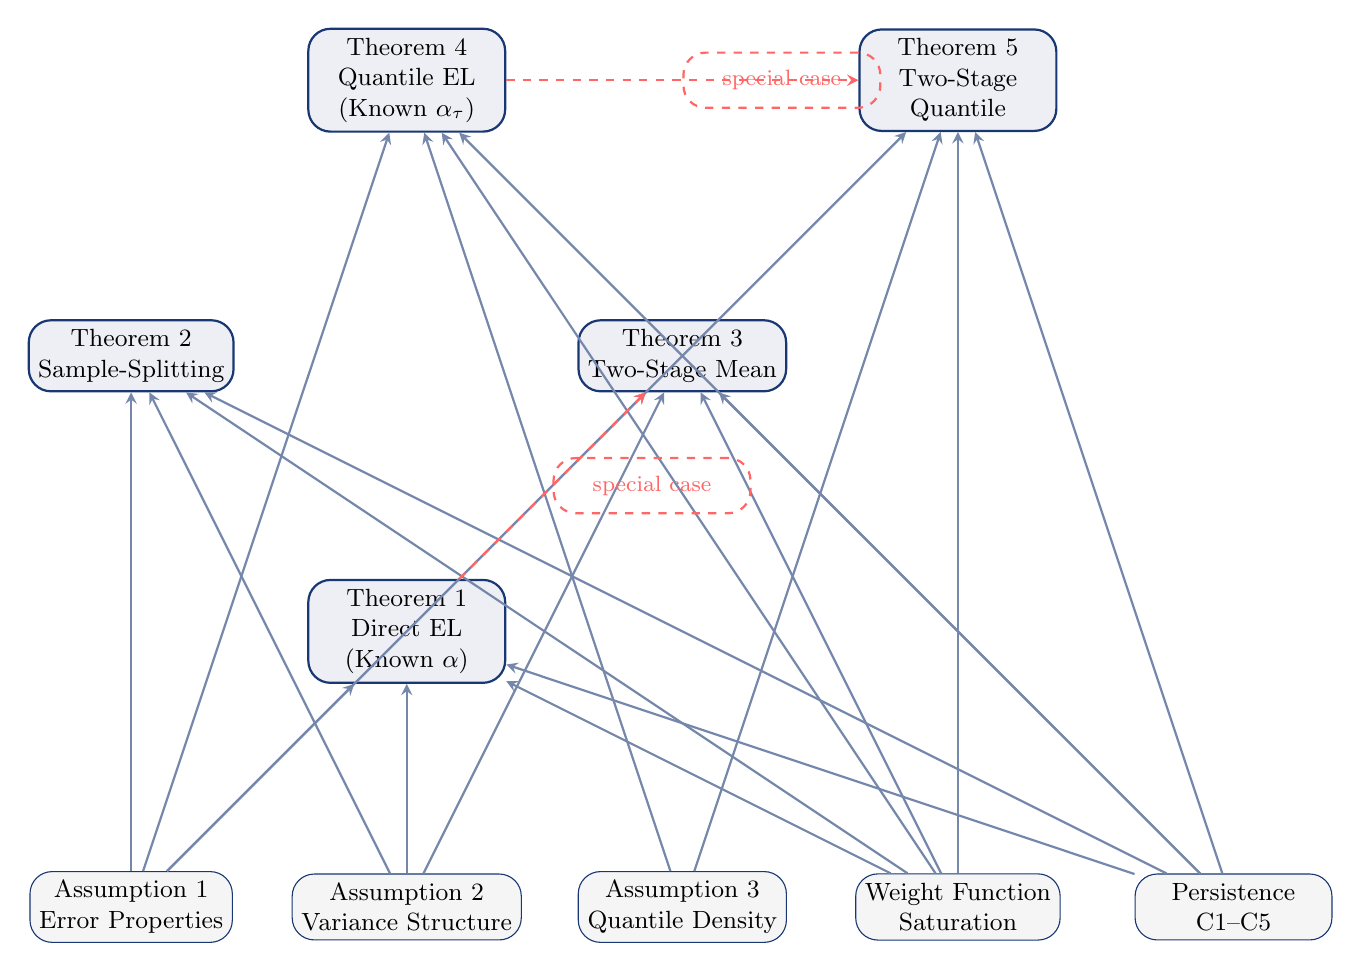
\begin{tikzpicture}[
    node distance=2.8cm and 1.8cm,
    every node/.style={draw, rounded corners=8pt, minimum width=2.5cm, minimum height=0.7cm, align=center, font=\small},
    asm/.style={fill=lightgray, draw=darkblue},
    thm/.style={fill=darkblue!8, draw=darkblue, thick},
    arr/.style={->, >=stealth, draw=darkblue!60, thick}
]
    % Assumptions (bottom layer)
    \node[asm] (A1) at (0,0) {Assumption 1\\Error Properties};
    \node[asm] (A2) at (3.5,0) {Assumption 2\\Variance Structure};
    \node[asm] (A3) at (7,0) {Assumption 3\\Quantile Density};
    \node[asm] (W) at (10.5,0) {Weight Function\\Saturation};
    \node[asm] (P) at (14,0) {Persistence\\C1--C5};

    % Theorems (upper layers)
    \node[thm] (T1) at (3.5,3.5) {Theorem 1\\Direct EL\\(Known $\alpha$)};
    \node[thm] (T2) at (0,7) {Theorem 2\\Sample-Splitting};
    \node[thm] (T3) at (7,7) {Theorem 3\\Two-Stage Mean};
    \node[thm] (T4) at (3.5,10.5) {Theorem 4\\Quantile EL\\(Known $\alpha_\tau$)};
    \node[thm] (T5) at (10.5,10.5) {Theorem 5\\Two-Stage\\Quantile};

    % Arrows: assumptions to theorems
    \foreach \t in {T1,T2,T3,T4,T5} {
        \draw[arr] (A1) -- (\t);
        \draw[arr] (P) -- (\t);
        \draw[arr] (W) -- (\t);
    }
    \draw[arr] (A2) -- (T1);
    \draw[arr] (A2) -- (T2);
    \draw[arr] (A2) -- (T3);
    \draw[arr] (A3) -- (T5);
    \draw[arr] (A3) -- (T4);

    % Arrows: theorem dependencies
    \draw[arr, dashed, red!60] (T1) -- (T3) node[midway, right, font=\footnotesize] {special case};
    \draw[arr, dashed, red!60] (T4) -- (T5) node[midway, right, font=\footnotesize] {special case};
\end{tikzpicture}
\caption{Logical dependency graph of the five theorems.
Solid arrows indicate direct dependence on assumptions.
Dashed red arrows indicate that one theorem is a special case of another
(Theorem~1 $\subset$ Theorem~3; Theorem~4 $\subset$ Theorem~5).}
\label{fig:dependency}
\end{figure}

%══════════════════════════════════════════════════════════════════
\section{Assumption-to-Claim Connections}
%══════════════════════════════════════════════════════════════════

\begin{table}[H]
\centering
\caption{Role of each assumption across theorems}
\label{tab:assumptions}
\begin{tabular}{p{3cm}p{6cm}p{5cm}}
\toprule
\textbf{Assumption} & \textbf{Role} & \textbf{Affected Theorems} \\
\midrule
A1 (Error properties) & Ensures martingale structure and moment bounds for CLT & All (1--5) \\
A2 (Variance structure) & Provides variance convergence for mean regression & 1, 2, 3 \\
A3 (Density regularity) & Enables Taylor expansion for quantile estimation & 4, 5 \\
Persistence (C1--C5) & Defines valid parameter space for $\rho_T$ & All (1--5) \\
Weight saturation & Handles nonstationarity via $w(x)^2 \to 1$ & All (1--5) \\
Weight centering & Eliminates intercept estimation error & 3, 5 \\
Sample-splitting ($m = \lfloor T/2 \rfloor$) & Removes intercept via differencing & 2 \\
Quantile martingale & Ensures $\psi_\tau(U_{t,\tau})$ is MDS & 4, 5 \\
\bottomrule
\end{tabular}
\end{table}

%══════════════════════════════════════════════════════════════════
\section{Finite-Sample Refinements}
%══════════════════════════════════════════════════════════════════

\subsection{Bartlett Bias Correction}

The paper proposes a Bartlett-type correction for the two-stage EL statistic:
\begin{equation}
    \widetilde{\ell}_T^{\,\text{BC}}(\beta_0) = \frac{\widetilde{\ell}_T(\beta_0)}{1 + \widehat{q}/T},
\end{equation}
where $\widehat{q} = \frac{1}{2}\widehat{\text{kurt}}(\widetilde{Z}_t) - \frac{1}{3}\widehat{\text{skew}}(\widetilde{Z}_t)^2$.

\subsection{Gradually Saturated Weights}

The paper reports new findings regarding the finite-sample impact of weight function choice:
\begin{itemize}
    \item The conventional weight $w_1(x) = x/\sqrt{1+x^2}$ can introduce distortions
    under high persistence due to its rapid saturation.
    \item The hyperbolic tangent weight $w_3(x) = \tanh(x/b)$ with small $b$
    provides \textbf{gradual saturation}, which stabilizes the EL constraint
    and reduces higher-order bias.
\end{itemize}

%══════════════════════════════════════════════════════════════════
\section{Empirical Application Highlights}
%══════════════════════════════════════════════════════════════════

The empirical analysis uses monthly U.S.\ stock market data (CRSP value-weighted index)
from January 1952 to December 2024, with 11 predictor variables.

\subsection{Mean Predictability}

Table~\ref{tab:empirical_mean} reproduces the key p-values for mean predictability tests.
A p-value below 0.05 indicates statistically significant predictability.

\begin{table}[H]
\centering
\caption{Empirical results for predictive mean regressions (selected variables)}
\label{tab:empirical_mean}
\begin{tabular}{lccc}
\toprule
\textbf{Predictor} & \textbf{EL2 (Sample-Splitting)} & \textbf{EL3 (Two-Stage)} & \textbf{IVX} \\
\midrule
Dividend-price ratio  & 0.93 & 0.21 & 0.29 \\
Earnings-price ratio  & 0.79 & 0.46 & 0.32 \\
Book-to-market ratio  & 0.85 & 0.66 & 0.53 \\
Treasury bill rate    & 0.04 & 0.03 & 0.02 \\
Long-term yield       & 0.11 & 0.11 & 0.08 \\
Inflation             & 0.01 & 0.03 & 0.01 \\
Default yield spread  & 0.66 & 0.29 & 0.30 \\
\bottomrule
\end{tabular}
\end{table}

\noindent\textbf{Key finding:} Mean predictability is modest and concentrated in
interest-rate-related variables (Treasury bill rate, inflation).
The two-stage EL3 generally shows stronger evidence than sample-splitting EL2.

\subsection{Quantile Predictability}

The quantile-based analysis reveals \textbf{substantially richer dynamics} across
the return distribution:

\begin{itemize}
    \item \textbf{Lower tails ($\tau = 0.1, 0.2$):}
    Treasury bill rate, long-term yield, and inflation exhibit strong predictability
    (p-values $< 0.05$), whereas dividend-based variables lose significance.

    \item \textbf{Upper tail ($\tau = 0.9$):}
    The default yield spread dominates (p-value $\approx 0$),
    while interest-rate variables become insignificant.

    \item \textbf{Center ($\tau = 0.5$):}
    Modest predictability, similar to the mean case.
\end{itemize}

This asymmetry highlights the value of quantile-based inference:
predictors that appear uninformative for the conditional mean may carry
strong signals in the tails of the return distribution.

%══════════════════════════════════════════════════════════════════
\section{Summary and Assessment}
%══════════════════════════════════════════════════════════════════

\subsection*{Theoretical Contributions}

\begin{enumerate}[leftmargin=*]
    \item \textbf{Unified $\chi^2$ limit theory} across five persistence regimes
    (C1--C5), including the previously uncovered mildly integrated (C2)
    and mildly explosive (C5) cases.
    \item \textbf{Relaxed error assumptions} compared to the existing EL literature:
    martingale differences with $\alpha$-mixing replace i.i.d.\ errors;
    conditional heteroscedasticity is fully accommodated.
    \item \textbf{Two complementary intercept-handling strategies}:
    sample-splitting (extended with relaxed conditions) and
    a novel two-stage procedure with centered weights.
    \item \textbf{Quantile extension} of EL inference,
    where sample-splitting is infeasible.
    \item \textbf{Practical finite-sample remedies}:
    Bartlett correction and gradually saturated weights.
\end{enumerate}

\subsection*{Limitations}

\begin{enumerate}[leftmargin=*]
    \item Single-predictor framework; multivariate extensions require
    additional theoretical development.
    \item The $\alpha$-mixing condition may be restrictive for some financial time series
    (e.g., those with long memory).
    \item Bartlett correction assumes approximate i.i.d.\ of $\widetilde{Z}_t$,
    which may not hold in practice.
\end{enumerate}

\subsection*{Connection to the FSM Research Project}

This paper shares several methodological connections with
the CGS (2025) paper previously analyzed in this project:

\begin{itemize}
    \item \textbf{Weight function approach}: Both papers use weight functions to handle
    nonstationarity, with the saturation property $w(x)^2 \to 1$ playing a central role.
    \item \textbf{Martingale CLT}: The core proof technique across both papers is the
    martingale central limit theorem with Lindeberg condition verification.
    \item \textbf{Assumption relaxation}: Both contribute to the broader project goal of
    understanding which regularity conditions are essential vs.\ relaxable.
    \item \textbf{Finite-sample concerns}: Both acknowledge the gap between asymptotic
    theory and finite-sample performance, proposing practical remedies.
\end{itemize}

%══════════════════════════════════════════════════════════════════
\section*{References}
%══════════════════════════════════════════════════════════════════

\begin{thebibliography}{99}

\bibitem{TwoStageEL2014}
Anonymous benchmark authors (2014).
A two-stage empirical likelihood method for predictive regressions.
\textit{Econometric Theory}, forthcoming.

\bibitem{BreakForecasting2023}
Anonymous benchmark authors (2023).
Nonparametric combination forecasting with structural breaks.
\textit{Working Paper}.

\bibitem{Choi2016}
Choi, Y., Jacewitz, S., and Park, J.Y.\ (2016).
A reexamination of stock return predictability.
\textit{Journal of Econometrics}, 192(1), 168--189.

\bibitem{DanglHalling2012}
Dangl, T.\ and Halling, M.\ (2012).
Predictive regressions with time-varying coefficients.
\textit{Journal of Financial Economics}, 106(1), 157--181.

\bibitem{FanLee2019}
Fan, R.\ and Lee, J.H.\ (2019).
Predictive quantile regressions under persistence and conditional heteroskedasticity.
\textit{Journal of Econometrics}, 213(1), 261--280.

\bibitem{GuKellyXiu2020}
Gu, S., Kelly, B., and Xiu, D.\ (2020).
Empirical asset pricing via machine learning.
\textit{Review of Financial Studies}, 33(5), 2223--2273.

\bibitem{HallHeyde1980}
Hall, P.\ and Heyde, C.\ (1980).
\textit{Martingale Limit Theory and its Application}.
Academic Press, Canberra.

\bibitem{Koenker2005}
Koenker, R.\ (2005).
\textit{Quantile Regression}.
Cambridge University Press.

\bibitem{Lee2016}
Lee, J.H.\ (2016).
Predictive quantile regression with persistent covariates: IVX-QR approach.
\textit{Journal of Econometrics}, 192(1), 105--118.

\bibitem{Owen1988}
Owen, A.B.\ (1988).
Empirical likelihood ratio confidence intervals for a single functional.
\textit{Biometrika}, 75(2), 237--249.

\bibitem{Owen1990}
Owen, A.B.\ (1990).
Empirical likelihood ratio confidence regions.
\textit{Annals of Statistics}, 18(1), 90--120.

\bibitem{Phillips2015}
Phillips, P.C.B.\ (2015).
Halbert White Jr.\ Memorial JFEC Lecture: Pitfalls and possibilities
in predictive regression.
\textit{Journal of Financial Econometrics}, 13(3), 521--555.

\bibitem{WelchGoyal2008}
Welch, I.\ and Goyal, A.\ (2008).
A comprehensive look at the empirical performance of equity premium prediction.
\textit{Review of Financial Studies}, 21(4), 1455--1508.

\bibitem{Xiao2009}
Xiao, Z.\ (2009).
Quantile cointegrating regression.
\textit{Journal of Econometrics}, 150(2), 248--260.

\bibitem{Zhu2014}
Zhu, F., Anonymous coauthor, and Peng, L.\ (2014).
Predictive regressions for macroeconomic data.
\textit{Annals of Applied Statistics}, 8(1), 577--594.

\end{thebibliography}

\medskip
\noindent\rule{\textwidth}{0.4pt}
\begin{center}
\small\textit{This analysis was automatically generated using the FSM Extraction Pipeline
(LangGraph-based) with DeepSeek LLM,}\\
\small\textit{then formatted as a human-readable \LaTeX\ document with enriched commentary.}
\end{center}

\end{document}
